%\vspace{-3mm}
\section{Introduction}
\label{sec.intro}
\noindent\textbf{Motivation.} Many data driven applications involve processing massive timeseries data, including IoT~\cite{cook2019anomaly}, medical AI~\cite{crabtree1990individual}, stock market~\cite{kraft1977determinants}, bank transactions~\cite{soro2020regular}, and so on. As such, there is a great need for timeseries analytics, such as trend recognition~\cite{shimakawa1992trend}, forecasting~\cite{chatfield2000time}, classification~\cite{ismail2019deep}, clustering~\cite{liao2005clustering}, similarity search~\cite{negi2005time}, and anomaly detection~\cite{teng2010anomaly}, with application ranging from identifying device failure~\cite{sun2019system}, automatically diagnosing diseases~\cite{bui2017time}, recognizing human activities~\cite{lara2012survey}, to stopping financial fraud~\cite{yue2007review}. 

To date, applications still mainly use traditional techniques such as ARIMA~\cite{arima}, TS-CHIEF~\cite{Shifaz2020TSCHIEFAS}, HIVE-COTE~\cite{10.1145/3182382}, and ROCKET~\cite{DBLP:journals/datamine/DempsterPW20}, to analyze timeseries data, which either heavily rely on humans to manually extract features based on their domain knowledge or are inadequate in handling complex multi-variate timeseries data.

A natural question is to ask whether deep learning -- which has revolutionized domains such as computer vision and natural language processing (NLP) -- could be applied.
To date, however, attempts to apply it to timeseries~\cite{DBLP:conf/kdd/ZerveasJPBE21} have not shown it to be universally superior, because deep learning requires extensive labeled examples and massive computational power to be effective.
In particular, despite the abundance of timeseries data in this ``Big Data'' era, the availability of labeled data is far more limited: extensive data labeling is often prohibitively expensive, as it typically requires a great deal of time and effort from domain experts.  

% \begin{figure}{}
% \vspace{-2mm}
%     \centering
%     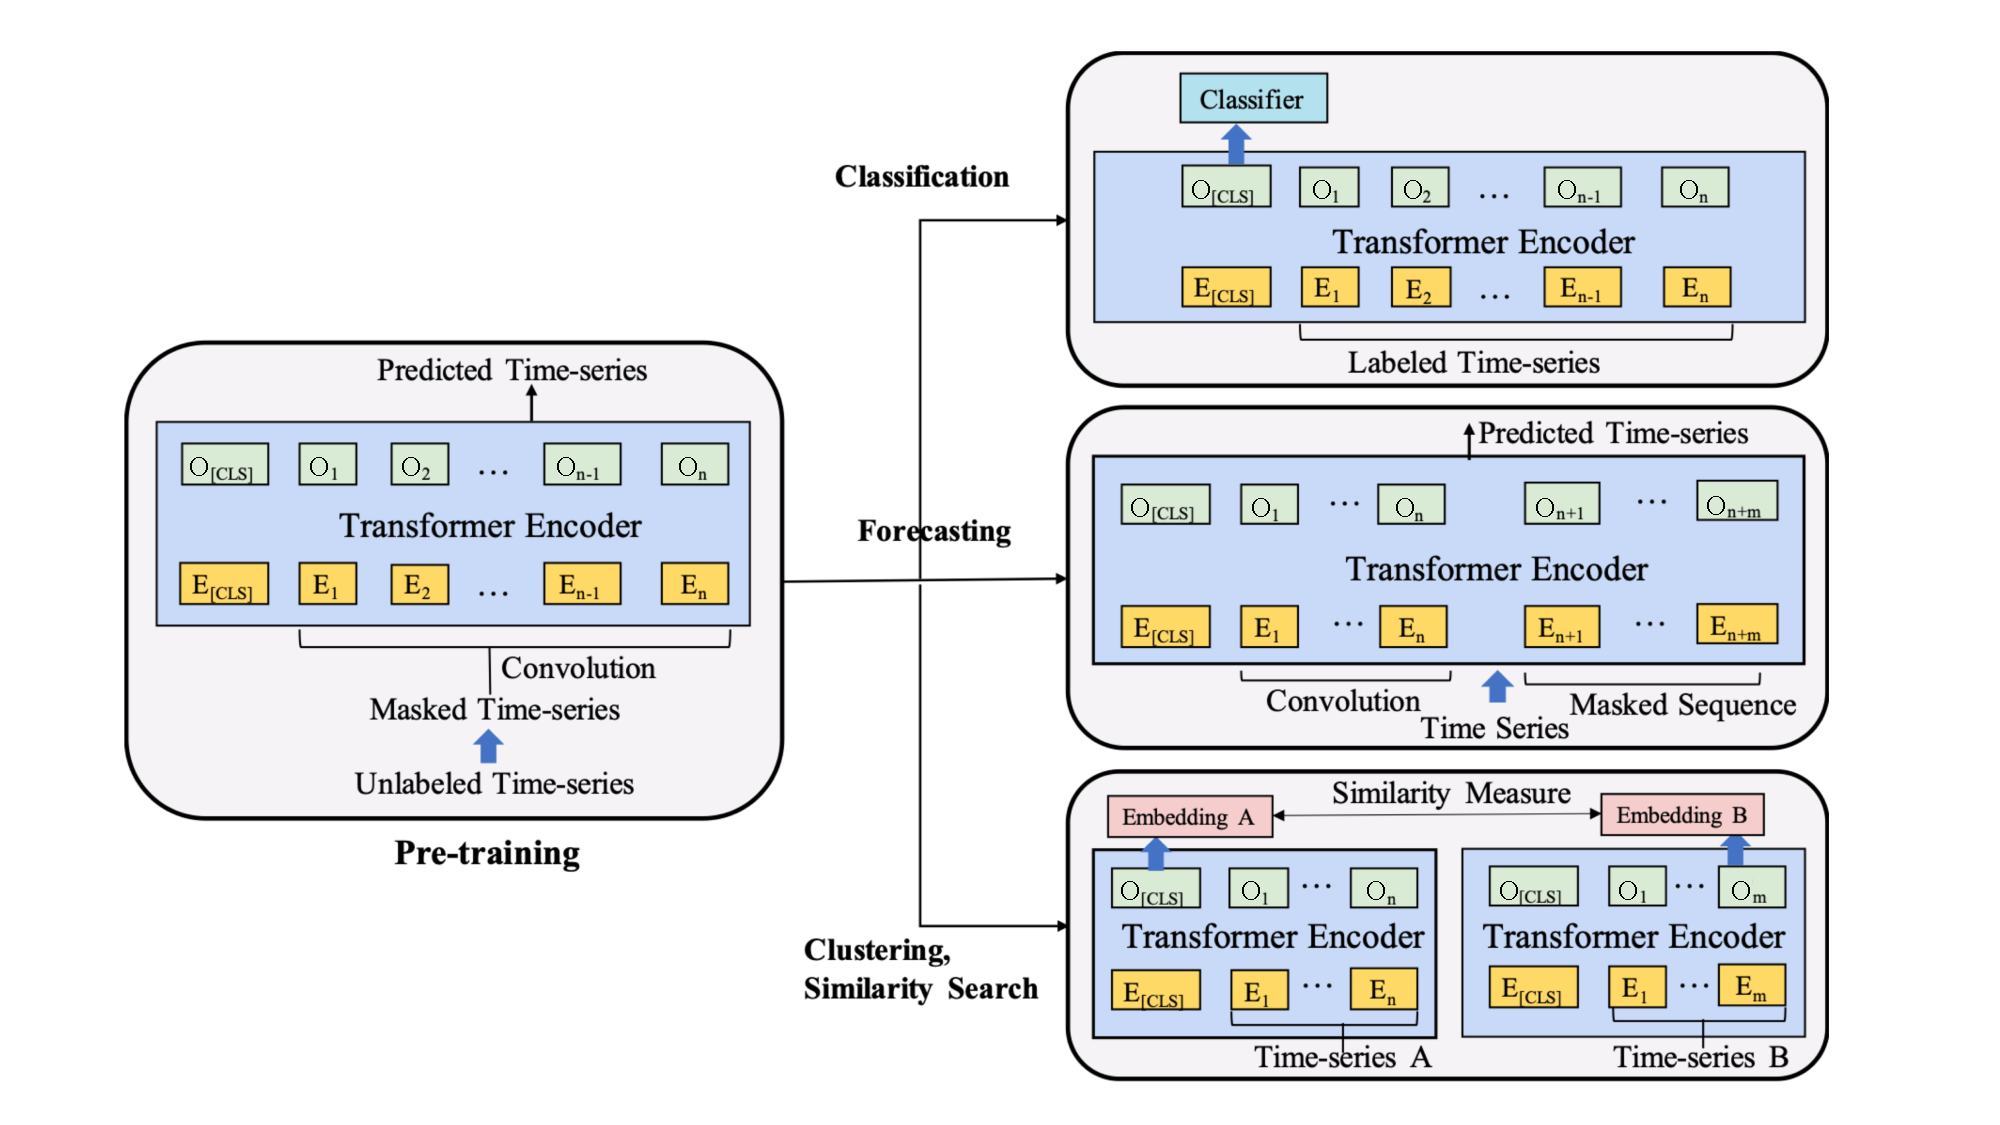
\includegraphics[width=1.0\columnwidth]{figures/overview.pdf}
%     \vspace{-7mm}
%     \caption{Overview of \system}
%     \label{fig.overview}
%     \vspace{-8mm}
% \end{figure}

%\vspace{-3mm}
\noindent\textbf{The \system Strategy.} 
We propose to tackle the aforementioned problems by building a general-purpose timeseries analytics tool that is {\bf automatic} -- freeing humans from manual feature extraction, {\bf self-supervised} -- requiring no labels while offering high accuracy by leveraging the existing plethora of unlabeled data, and {\bf scalable} -- efficiently handling highly complex, massive-scale timeseries data. 

The key observation is that in timeseries data, the sequential order among the values (stock trading price, volume, etc.) over time matters. That is, each value is highly correlated with other values observed before or after it. 
This fundamental property of timeseries bears similarity to natural language at a high level, where a word is correlated to other words in each sentence.  
Inspired by the {\it mask and predict} methodology used in Bert~\cite{DBLP:conf/naacl/DevlinCLT19} which has been remarkably successful in natural language processing (NLP)~\cite{DBLP:conf/naacl/DevlinCLT19}, we developed a {\it self-supervised} pre-training method, called \system, to train a deep learning model which takes the correlations among different observations into consideration. 

%Fig.~\ref{fig.overview} shows an overview of \system. 
Given a collection of {\it unlabeled} timeseries, \system first pre-trains a Transformer model which {\it automatically} produces high quality feature embeddings for timeseries data. This pre-trained model are then used to support various downstream tasks. For example, as with BERT, \system supports {\it supervised tasks} such as classification by fine-tuning the pre-trained parameters to achieve high accuracy with {\it small number} of labels.
\system also naturally supports other {\it analytics} tasks such as forecasting, missing value imputation, and outlier detection. \system automatically produces feature embeddings by randomly masking some of the values from the input timeseries and predicting the masked values based on their contexts. It thus can be used to directly impute missing values and future values, while outliers can be identified as the observations that significantly deviate from their corresponding predictions~\cite{10.1007/978-3-030-77964-1_17}. {\it Unsupervised analytics tasks} such as clustering and similarity search can run directly on the feature embeddings produced by \system, which encode the long term trends of the timeseries and tend to be more informative than the raw features traditionally used in modeling the similarity of different timeseries objects~\cite{DBLP:conf/kdd/WangP21}.

%\vspace{-3mm}
\noindent\textbf{Scalability Challenge.} The key challenge is to make \system scalable to long timeseries.
The idea of self-attention~\cite{DBLP:conf/nips/VaswaniSPUJGKP17} is central to pre-training methods in NLP. Self-attention computes the pairwise correlations among different semantic units in a sentence, and as such, has {\it quadratic} time and space complexity in the length of the input sequence. 
This limits the model's scalability, especially when handling large-scale timeseries data, which is common in real-world applications such as IoT, medical AI, and finance~\cite{zhou2021informer,DBLP:journals/pvldb/CaoTAJYLGSBSCWM19,liu2018open}. Predictions about timeseries may need to look at months or years of historical data to make accurate predictions, spanning hundreds of thousands of samples.  
As a concrete example, in collaboration with a research hospital we have been developing a seizure classifier~\cite{DBLP:journals/pvldb/CaoTAJYLGSBSCWM19} that automatically detects seizures based on EEG signals (timeseries) collected during the clinical observation of patients. As seizures last only a few seconds, we chunk long EEG data into many 2 second segments and detect seizures at a segment level. However, the classification of a particular segment depends on up to 12 hours of prior signal to determine if one 2 second segment indicates seizure or not, because seizure diagnosis needs to consider the long-term trend of the EEG data. The number of segments in 12 hours is more than 21k. 
This is far larger than the number of semantic units the typical NLP tasks expect. For example, BERT~\cite{DBLP:conf/naacl/DevlinCLT19} limits the number of units to 512 \srm{and even massive models like GPT-3 limit the number of units to XXX}.
Existing works~\cite{DBLP:conf/kdd/ZerveasJPBE21} directly apply Transformers to process timeseries data and thus are not scalable to such long inputs. 
Although in NLP some lower complexity methods have been proposed to {\it approximately} compute self-attention~\cite{kitaev2020reformer,choromanski2020rethinking,wang2020linformer}, their performance degrades dramatically when used on timeseries due to the gap between natural language and timeseries, as shown in our experiments. 

%This is far more than the number of semantic units the typical NLP tasks expect. For example, GPT-3, which took tens of years of GPU time to train, limits the number of units to 2048.
%\vspace{-3mm}
\noindent\textbf{Proposed Approach.} 
To scale \system to long timeseries, we  propose a novel attention mechanism, called {\bf group attention}. Leveraging the periodicity of timeseries, \system chunks the timeseries into segments and dynamically clusters the segments of each input timeseries into a small number of groups, where the segments in the same group have similar feature embeddings during the current training iteration and thus can share the attention computation. The longer the timeseries is, the more sharing opportunities it offers.
\system then computes the self-attention at the group level.
In this way, group attention produces a {\it compressed attention matrix} and eliminates both the CPU and memory bottleneck in transformer-style models, thus scalable to long timeseries.

Moreover, to preserve the accuracy on the downstream tasks, we design an {\it embedding aggregation} strategy and a customized {\it group softmax function} which together ensure \system is still able to produce high quality feature embeddings using this compressed attention matrix. 
We design GPU friendly strategy to group the segments {\it in parallel}, effectively minimizing the grouping overhead.

\textbf{Adaptive Scheduling.}
In \system, {\it the number of groups} $N$ balances the speed up and the quality of attention approximation. A small $N$ will lead to a large speed up, but potentially large approximation errors. On the other hand, although a large $N$ tends to produce high-quality approximations, it inevitably slows down the training process. Therefore, an appropriate $N$ is critical to the performance of group attention. However, $N$ depends on the distributional properties of the datasets. Furthermore, like the classical transformer models, \system stacks multiple attention layers to produce better embeddings. Different layers should also use different values of $N$. 
This makes manually setting an appropriate $N$ almost impossible. 

To solve this problem, we propose an adaptive scheduling strategy which dynamically decides an appropriate $N$ in the training process. It starts with a large $N$ and iteratively merges groups that are similar to each other. Guided by an error bound on the approximated self-attention that users can tolerate, it automatically determines if two groups are mergeable, performing merging efficiently in a GPU-friendly way. 

\textbf{Batch Size.} As \system adjusts $N$ dynamically during training, a fixed batch size raises problems: as $N$ decreases, the memory usage of a single sample decreases. This allows a larger batch size which is beneficial, because: 
(1) it makes full use of GPU memory; (2) high-parallelism across the samples in a big batch brings better performance. 
Our experimental study shows that doubling the batch size reduces the training time by 30\%, while still preserving the quality of the model. Thus, \system should dynamically adjust batch-size as $N$ changes.

We thus propose a learning-based method to model the correlation between the number of groups $N$ and the batch size $B$. The model is then used to predict $B$ for a given $N$ when training \system.
More specifically, we first sample some $N$ values in a reasonable range. For each sampled $N$, we find a batch size that consumes up to a certain percentage of GPU memory in a cost-efficient way. Using a small set of mathematical functions as prior, \system learns the model with only a few <N, B> pairs as ground truth labels.    

Our experiments on public timeseries benchmarks and the MGH EEG data~\cite{DBLP:journals/pvldb/CaoTAJYLGSBSCWM19} confirm that \system outperforms the state-of-the-art methods in accuracy on various timeseries analytics tasks, while our group attention mechanism achieves a 63X speedup with much less memory required, compared to the existing self-attention mechanisms~\cite{DBLP:conf/nips/VaswaniSPUJGKP17,choromanski2020rethinking,wang2020linformer}.

\noindent\textbf{Contributions.} The key contributions of this work include:

\begin{compactitem}
\item We build \system, a general-purpose timeseries analytics tool that is automatic, self-supervised, scalable to high complexity, massive-scale timeseries data.

% \item We design a time-aware convolution operation to bridge the gap between timeseries and natural language. 

\item Leveraging the periodicity of timeseries, our group attention mechanism reduces the time and space complexity of the self-attention mechanism with accuracy guarantees, allowing  \system to scale to long timeseries data.

\item Guided by an approximation error bound, our adaptive scheduler dynamically adapts the number of groups and the batch size to the distribution properties of the evolving feature embeddings, making group attention efficient and easily tuning.

\item We conduct experiments on various datasets and different analytics tasks, confirming that \system is up to 63 times faster than the state-of-the-art, yet better in accuracy. 

\end{compactitem}
